\item Una lista con la venta promedio, venta total, mayor venta, menor venta, y total de órdenes, por región, estado y ciudad. La venta promedio debe estar entre \$900 y \$1,500.

\begin{lstlisting}
detalle = customer ⨝ orders ⨝ products

importes = π region,state,city,orderid,(quantity * price) -> importe (detalle)

ventas = γ region,state,city,orderid; sum(importe)→venta (importes)

resumen = γ region,state,city; avg(venta)→promedio, sum(venta)→total, max(venta)→mayor, min(venta)→menor, count(orderid)→ordenes (ventas)

resultado = σ promedio ≥ 900 ∧ promedio ≤ 1500 (resumen)

τ region ASC,state ASC,city ASC (resultado)
\end{lstlisting}

\begin{figure}[h]
\centering
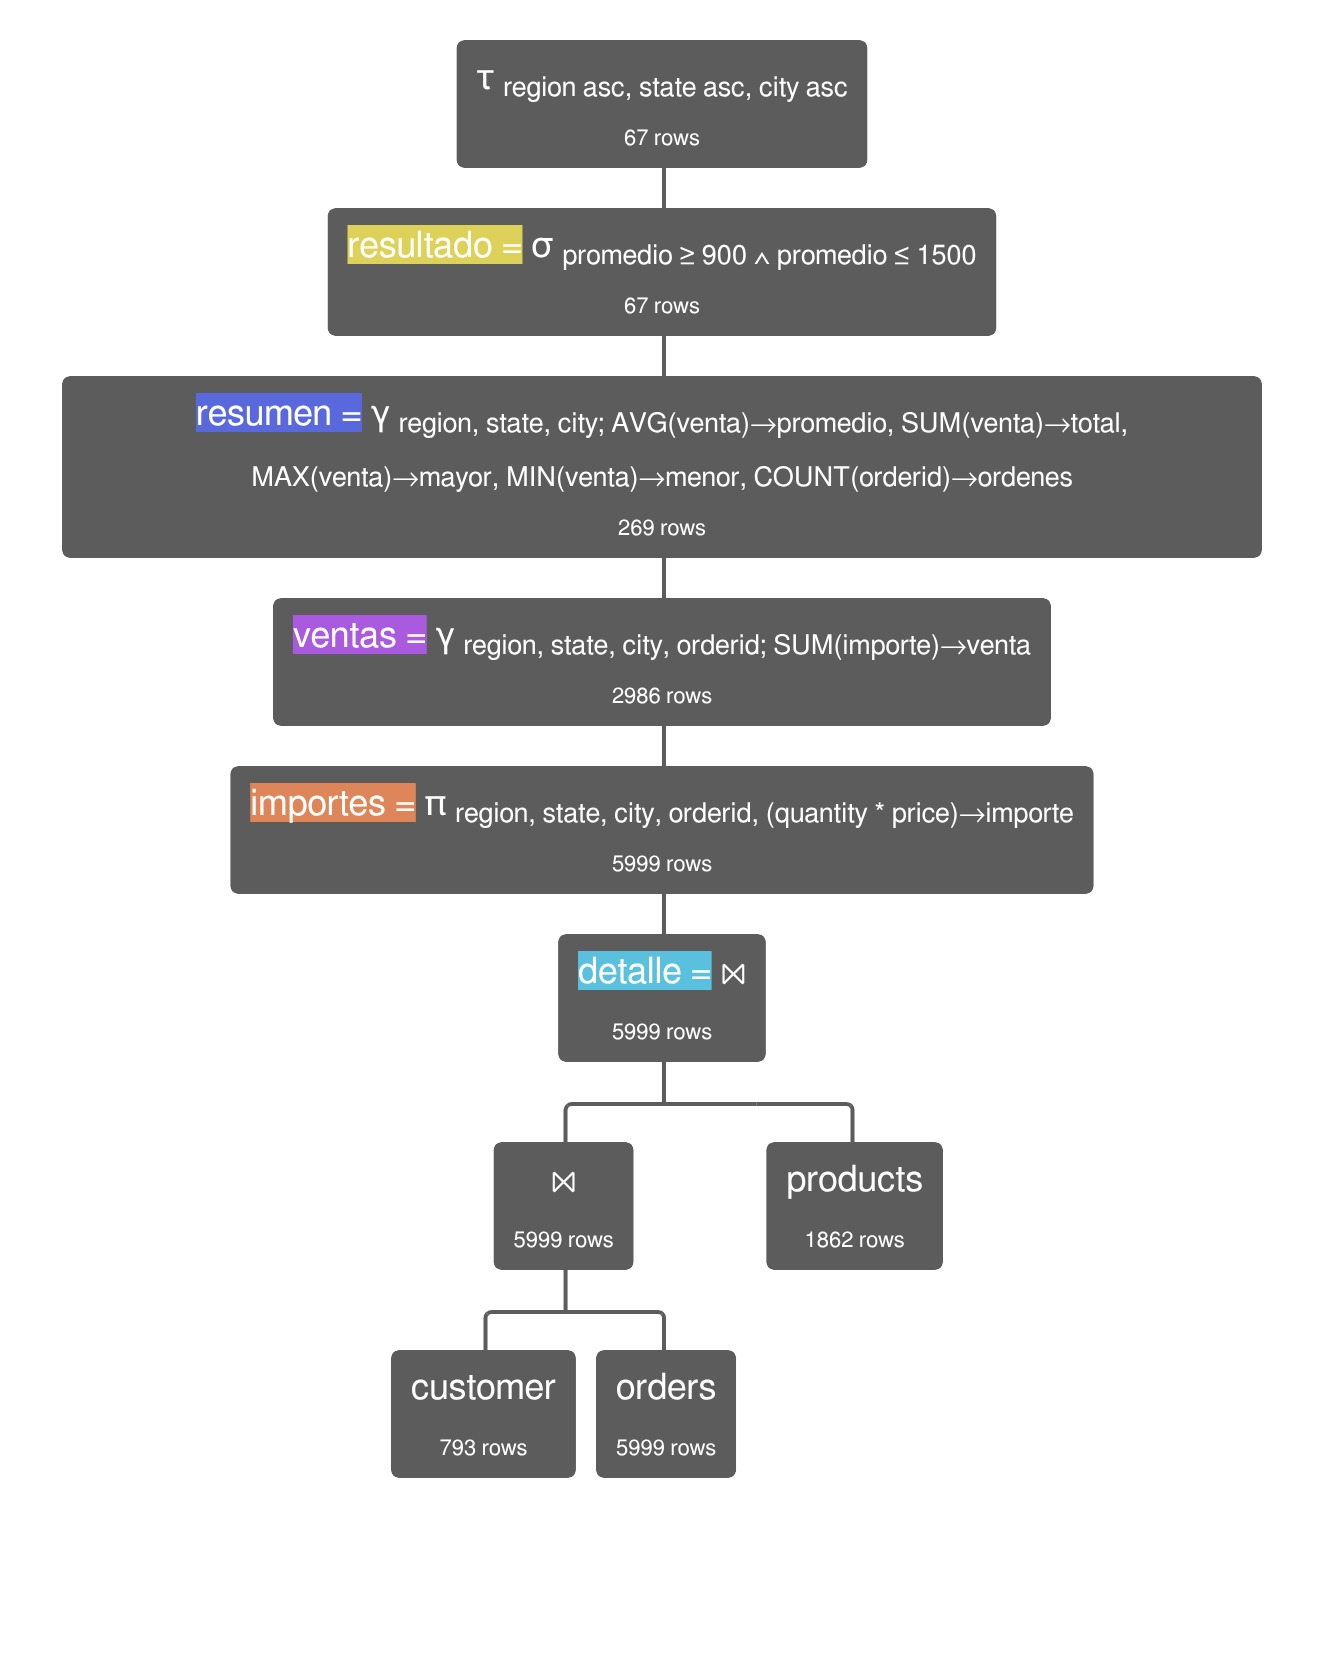
\includegraphics[width=0.5\textwidth]{figuras/2h_1.jpg}
\end{figure}

\begin{figure}[h]
\centering
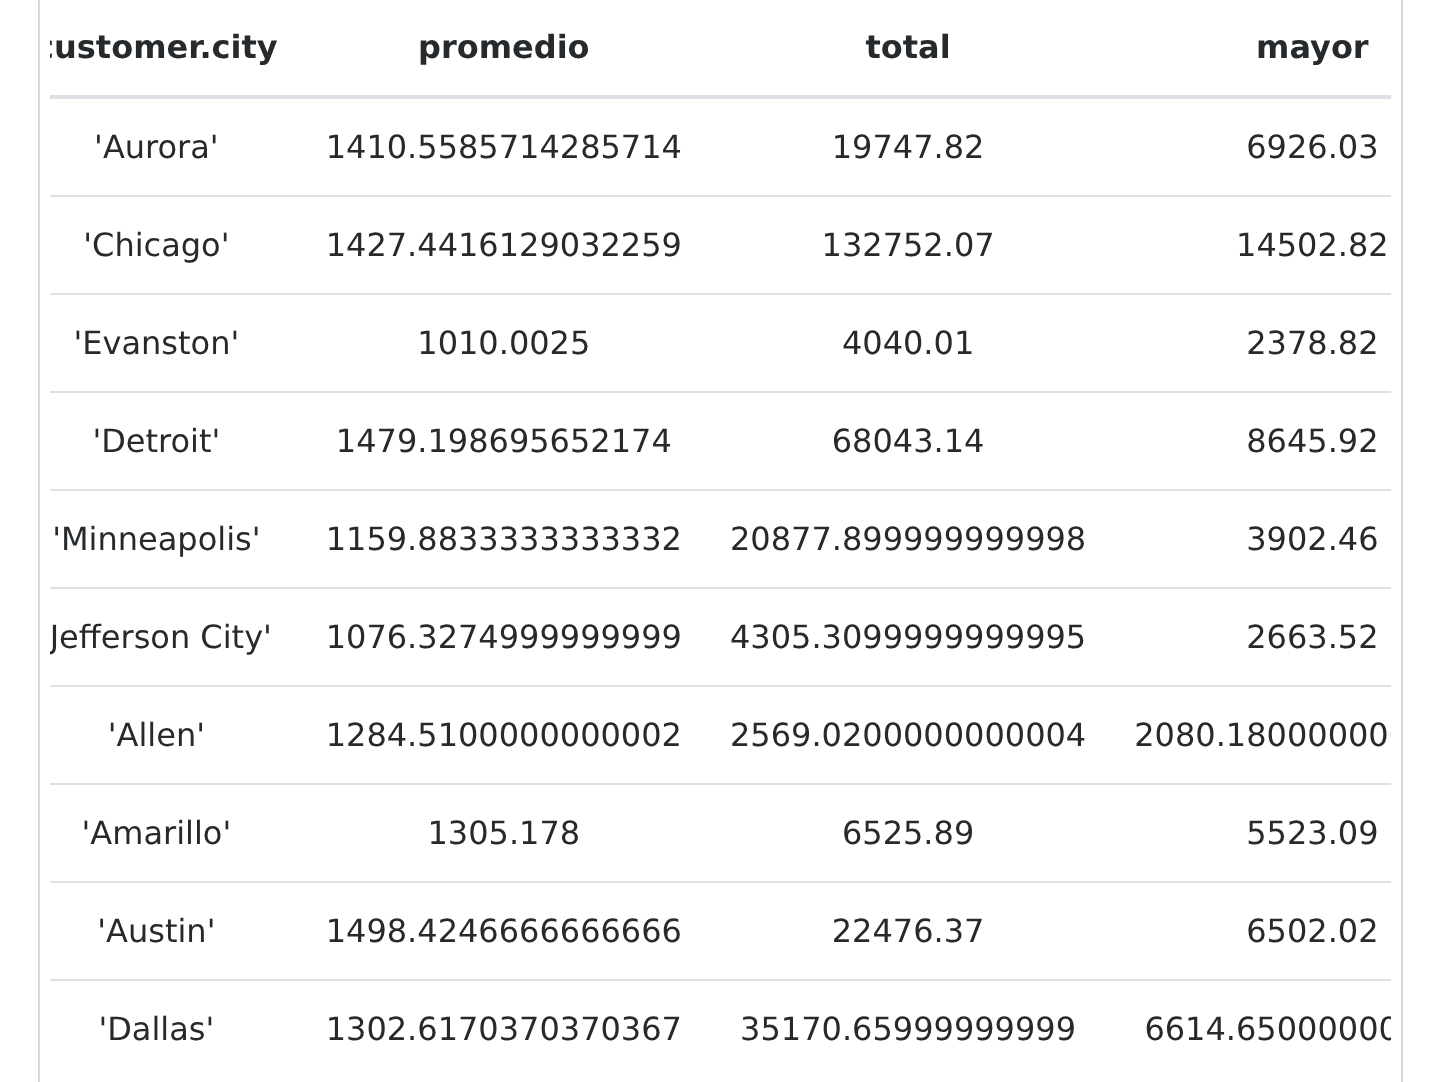
\includegraphics[width=0.3\textwidth]{figuras/2h_2.png}
\end{figure}

\newpage